\section{Theorie}
\label{sec:Theorie}

\subsection{Grundlagen Laser Physik}
\label{sec:Grundlagen}
Das englische Synonym Laser steht für \textit{light amplification by stimulated emission of radiation}
und bezeichnet den physikalischen Effekt, mit dem  Laserstrahlen erzeugt werden.
Im Unterschied zu anderen Lichtquellen emittieren Laser Licht der gleichen Wellenlänge, Phase, Polarisation und Richtung. 
Daher Stellen sie in der Experimentalphysik ein wichtiges Instrument dar,
zum Beispiel bei der Untersuchung von Materialien.

Ein Laser besteht typischerweise aus drei Bauteilen. Das \textit{aktive Medium}, die \textit{Pumpe} und den \textit{Resonator}.
Im aktiven Medium werden durch Quantensprünge von Elektronen auf niedrigere Energie Niveaus Photonen emittiert.
Diese Abfallen auf niedrigere Niveaus kann verschieden ablaufen (vgl. Abbildung \ref{fig:emmision}).
\begin{figure}[h]
    \centering
    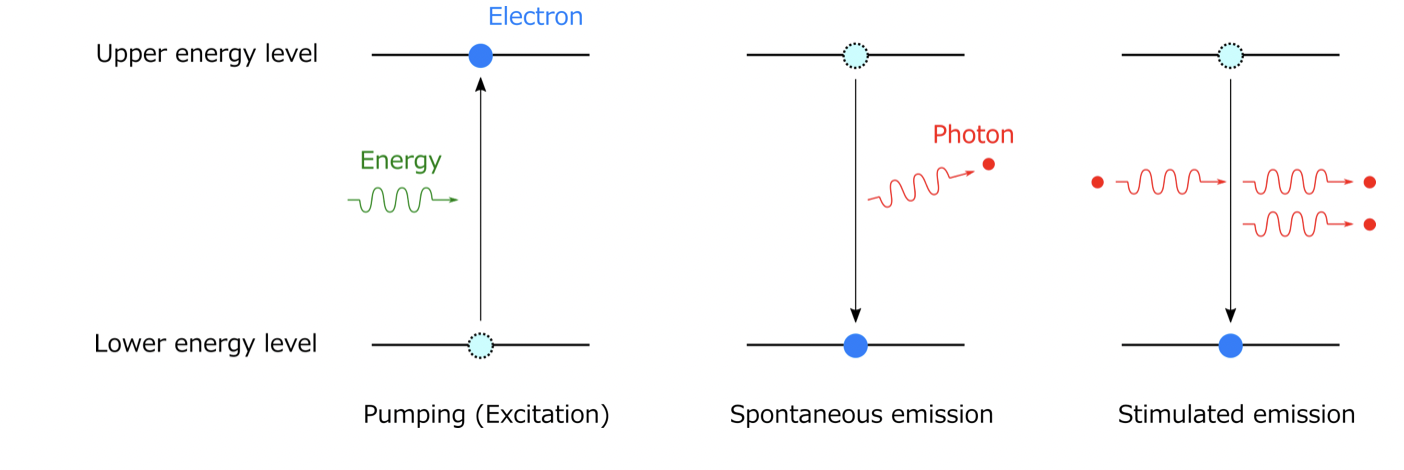
\includegraphics[width=0.7\textwidth]{abb/emission.png}
    \caption{Absorption spontane Emission und stimulierte Emission \cite{emission}}
    \label{fig:emmision}
\end{figure}
Um monochromatische, kohärente Strahlung zu emittieren, ist besonders die stimulierte Emission von Bedeutung,
da bei der spontanen Emission, Richtung und Phase des emittierten Photons zufällig auftreten.
Bei der stimulierten Emission hingegen fällt das Elektron erst durch die Stimulation eines Photons auf das niedrigere Energieniveau,
dabei wird ein Photon mit exakt denselben Eigenschaften wie die des Stimulierende Photon erzeugt.
Das so entstandene zweite Atom kann nun selber andere Elektronen stimulieren,
sodass es zu einer Kettenreaktion kommt. 
Durch den Resonator, 
welcher meist aus zwei Spiegeln besteht,
die mit passendem Abstand zur Wellenlänge positioniert sind,
sodass sich eine stehende Welle bildet,
durchlaufen die Photonen das Lasermedium mehrmals,
was die Chance, ein weiteres Elektron zu stimulieren, erhöht. 
Einer der beiden Spiegel ist lichtdurchlässig, wodurch die Photonen zur Nutzung austreten können.
Um das Prinzip der stimulierten Emission nutzen zu können,
muss im aktiven Medium ein Zustand der Besetzungsinversion hergestellt werden.
Also, 
dass der energiereichere Zustand mit höherer Wahrscheinlichkeit besetzt ist als der Energie niedrigere.
In einem zwei Zustand System kann eine solche Besetzungsinversion nicht hergestellt werden,
da sich Absorption und stimulierte Emission gerade ausgleichen. 
Erst mit einem dritten Energieniveau (vgl. Abbildung \ref{fig:dreiniveau}) ist eine Besetzungsinversion möglich.
\begin{figure}[h]
    \centering
    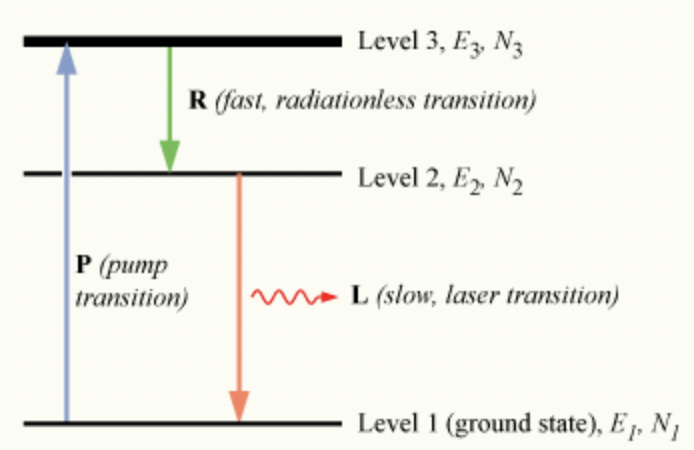
\includegraphics[width=0.5\textwidth]{abb/dreiniveau.png}
    \caption{Besetzungsinversion im drei-Zustandssystem \cite{enwiki}}
    \label{fig:dreiniveau}
\end{figure}
Die Elektronen werden vom System von Niveau 1 auf Niveau 3 gepumpt. 
Dort gehen sie weitgehend strahlungsfrei in Niveau 2 über, 
um dann durch stimulierte Emission wieder in Niveau 1 zu fallen.
Da der Pump Vorgang nicht das mittlere Niveau anspricht,
kann dort eine höhere Besetzungszahl erzeugt werden. 


\subsection{External Cavity Diode Lasers (ECDL)}
\begin{figure}[h]
    \centering
    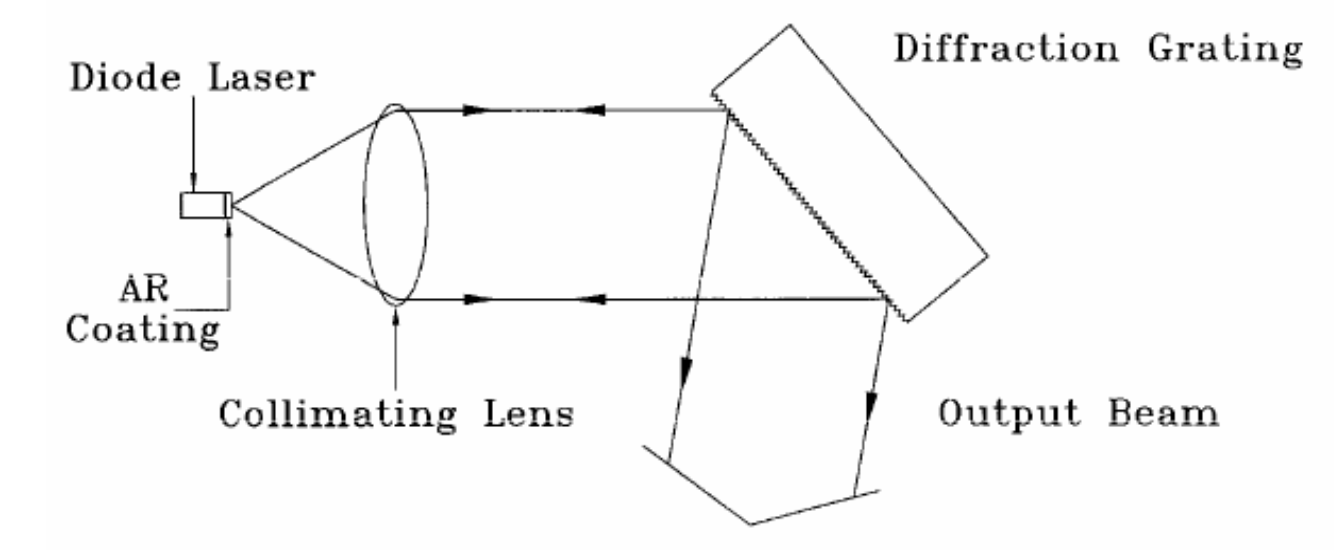
\includegraphics[width=0.8\textwidth]{abb/Aufbau.png}
    \caption{Schematischer Aufbau eines ECDL \cite{laser}}
    \label{fig:aufbau}
\end{figure}
In der Abbildung \ref{fig:aufbau} ist ein schematischer Aufbau des verwendeten Diodenlasers zu sehen.
Der eigentliche Diodenlaser besteht jeweils aus einer p- und n-dotierten Schicht.
Der pn-Übergang bildet das aktive Medium, 
welches nach dem in Kapitel \ref{sec:Grundlagen} beschriebenen Prinzip Photonen emittiert,
die wie ebenfalls in Kapitel \ref{sec:Grundlagen} beschrieben im (internen) Resonator eine stehende Welle bilden.
Der durch den halbdurchlässigen Spiegel austretender Anteil wird durch eine Kollimator-Linse gelenkt
und trifft anschließend auf ein optisches Gitter (Diffraction Grating),
das gerade so justiert ist 
das dass Beugungsmaximum nullter Ordnung aus dem Laser gelenkt wird.
Höhere Ordnungen werden wieder zur Diode hin reflektiert,
wodurch sich eine weitere stehende Welle bildet, 
zwischen Gitter und undurchlässigen Spiegel.
Dies ist der externe Resonator.

\subsection{Laserabstimmung}
Die einzelnen Komponenten tragen abhängig von der Wellenlänge $\lambda$ zur Netto-leistung bei.
\begin{figure}[h]
    \centering
    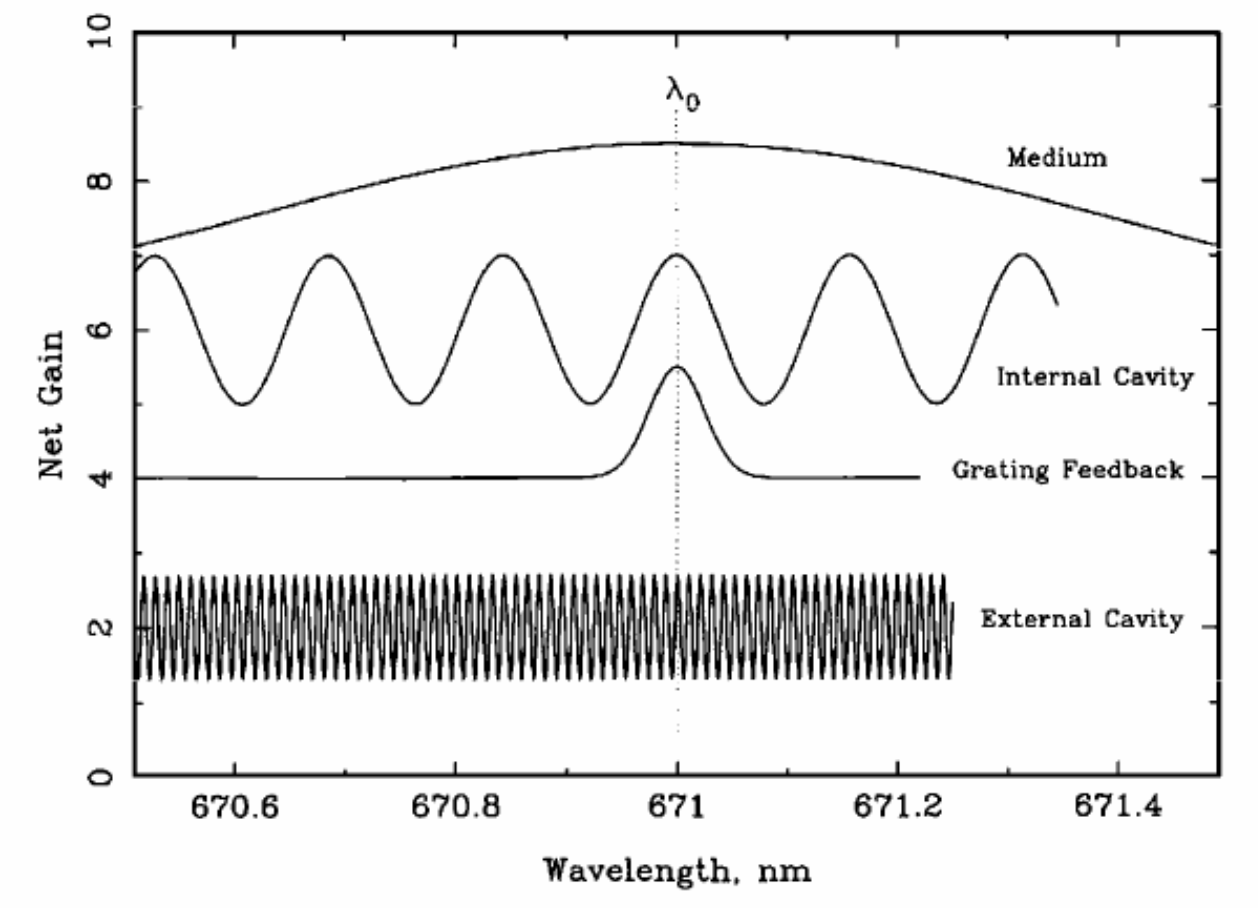
\includegraphics[width=0.8\textwidth]{abb/Laserabstimmung.png}
    \caption{Anteile der verschiedenen Komponenten. Zu Gunsten der Lesbarkeit sind die Graphen versetzt zueinander aufgetragen \cite{laser}}
    \label{fig:komponenten}
\end{figure}
In Abbildung \eqref{fig:komponenten} sind die verschiedenen Beiträge der Komponenten aufgetragen.
Das aktive Medium hat sein Maximum gerade bei der Größe der Bandlücke des Halbleiter-Materials.
Da sich die Elektronen nicht in diskreten Energien,
sondern in Energiebändern aufhalten, ist das Maximum des Mediums ebenfalls nicht diskret.
Strom und Temperatur beeinflussen ebenfalls den Beitrag des aktiven Mediums,
indem sie den Peak, also die emittierte Wellenlänge, verschieben.
Das optische Gitter besitzt, 
wie zu erwarten,
nur ein Peak,
da andere Wellenlängen in andere Richtungen gestreut werden. 
Die beiden stehenden Wellen der Resonatoren sind ebenfalls zu erkennen.
Es werden gerade die Wellenlängen verstärkt,
deren ganzzahliges Vielfaches die Resonatorlänge $L$ ergibt
\begin{equation*}
    L = \frac{\lambda}{2}N.
\end{equation*} 
Durch die unterschiedlichen Resonatorlängen ergeben sich auch die verschiedenen Frequenzen in der Abbildung.

Addiert man die verschiedenen Netto Leistungen ergibt sich eine Gesamt Netto Leistung wie in Abbildung \ref{fig:netto}.
\begin{figure}
    \centering
    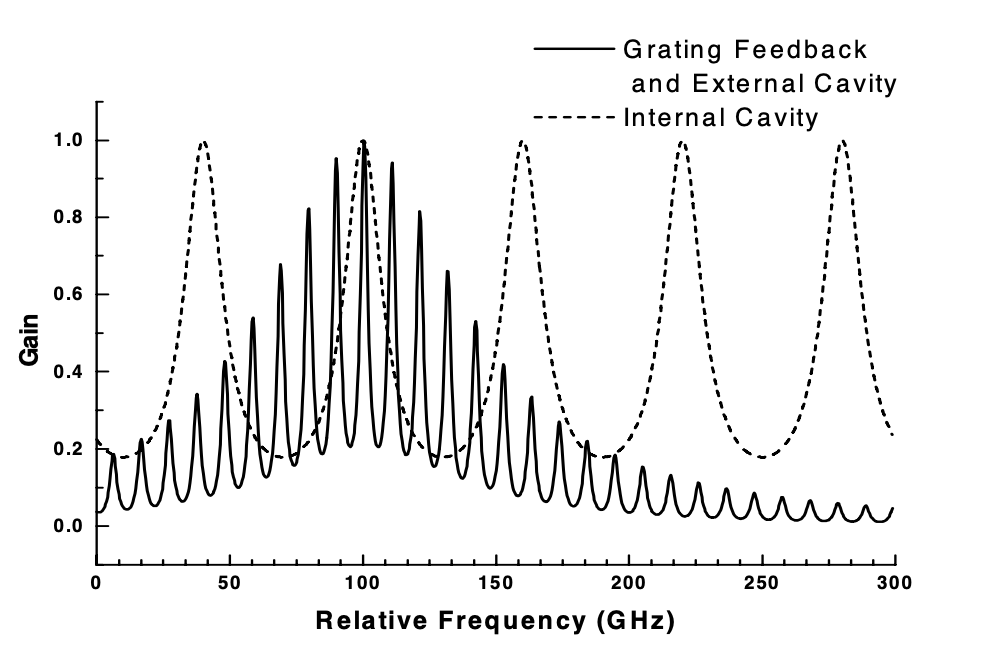
\includegraphics[width=0.7\textwidth]{abb/netto.png}
    \caption{Einfluss der beiden Resonatoren und des Gitters \cite{laser}}
    \label{fig:netto}
\end{figure}

\subsection{Mode Hops}
Da es für die weitere Verwendung des Lasers wichtig ist,
dass das Laserlicht nur eine Wellenlänge besitzt,
gilt es sogenannte \textit{Mode Hops} zu verhindern.
Sie entstehen, 
wenn externer und interner Resonator so aufeinander eingestellt sind,
dass zwei verschiedene Wellenlängen verstärkt werden (vgl. Abbildung \ref{fig:modehops}).
\begin{figure}
    \centering
    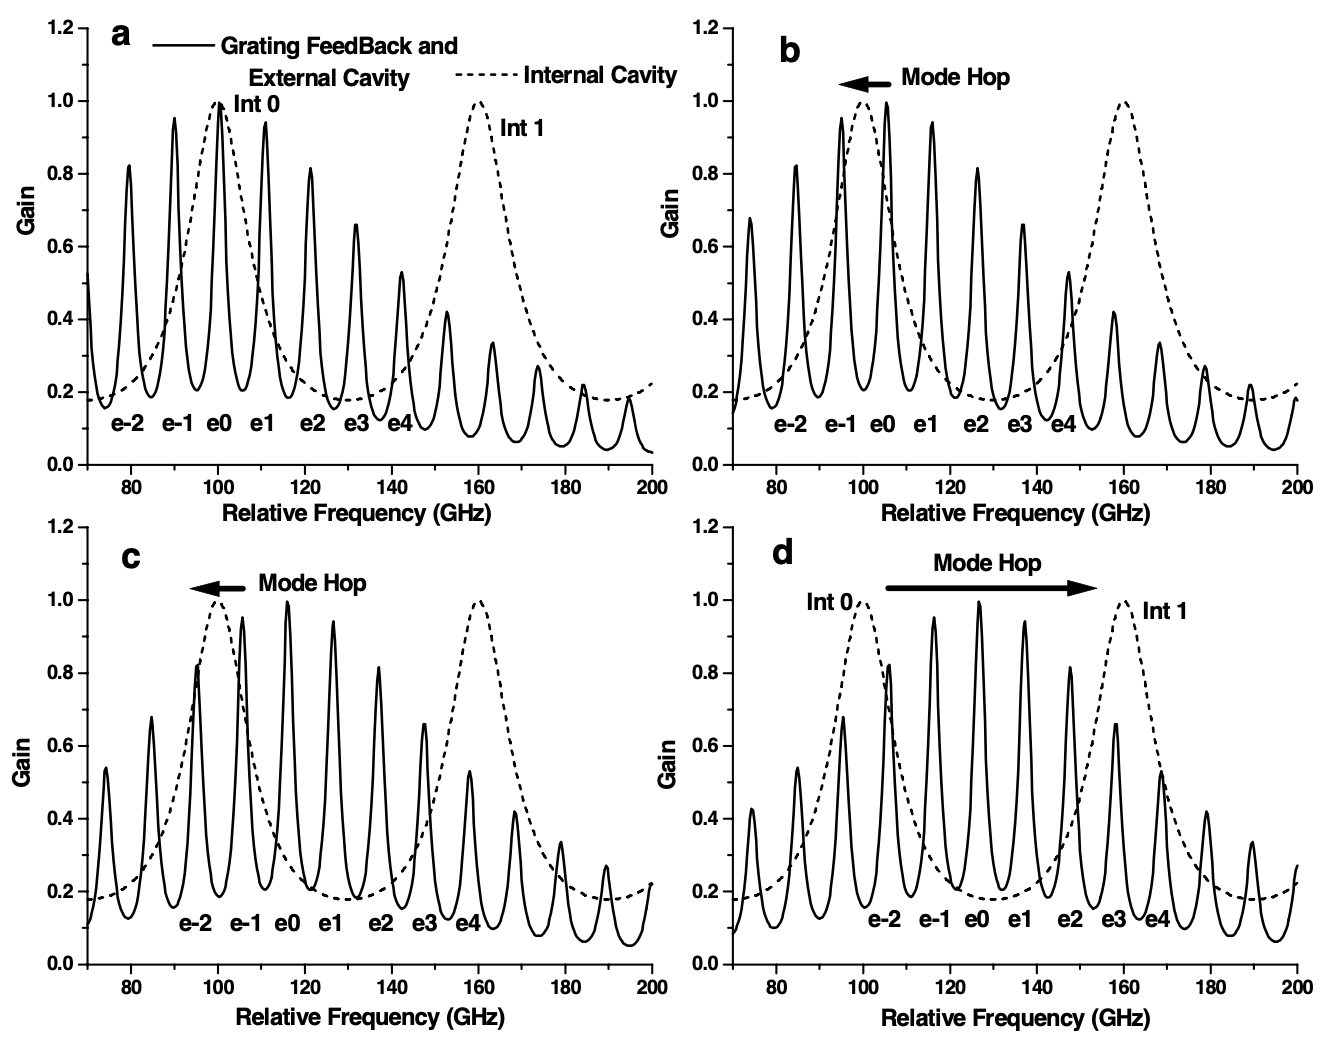
\includegraphics[width=0.7\textwidth]{abb/modehops.png}
    \caption{Darstellung verschiedener Mode Hops \cite{laser}}
    \label{fig:modehops}
\end{figure}
In Darstellung \textbf{A} ist erkennbar, das sowohl der externe wie auch der interne Resonator eine Wellenlänge deutlich verstärken.
Verschieben sich die Verhältnisse
wie in den Abbildungen \textbf{B} bis \textbf{D} dargestellt,
addieren sich zwei verschiedene Wellenlängen.
Zur Folge hat dies einen willkürlichen Sprung zwischen den beiden Wellenlängen in der Nettoleistung.
Daher ist bei der Einstellung der Resonatoren besonders auf die Vermeidung solcher Mode Hops zu achten.



